\documentclass[11pt]{article}
\usepackage[czech]{babel}
\usepackage{cite}
\usepackage[utf8]{inputenc}
\usepackage{titling}
\usepackage{graphicx}
\usepackage[nodayofweek,level]{datetime}
\newcommand{\mydate}{\today}
\usepackage{url}
\usepackage{float}
\usepackage{geometry}
\usepackage{pdflscape}

\let\endtitlepage\relax

\newcommand{\subtitle}[1]{%
  \posttitle{%
    \par\end{center}
    \begin{center}\large#1\end{center}
    \vskip0.5em}%
}

\begin{document}

\begin{center}
        {\Huge
        \textsc{Vysoké učení technické v Brně} \\
        \medskip
      \huge{\textsc{Fakulta informačních technologií}}
         }\\
      \end{center}
      
  \vspace{10pt}      	
     
    
  \vspace{40pt}	  	
    
    \begin{center}
    {\Huge
    \textsc{Modelování a Simulace}
    }
    
    \vspace{20pt}		
      
    {\Huge
      \textbf{Výrobní proces z potravinářské oblasti}
    }

    \vspace{50pt}			
    

    
    \end{center}
  	
    
    {\Large 
      Jan Bartošek (xbarto92) \hfill Brno, \mydate
      \newline \par
      Petr Šopf (xsopfp00)
    }	  	

    \vspace{150pt}


\section{Úvod}
Tato práce vznikla za účelem projektu do předmětu Modelování a simulace, Fakulty informačních technologií vysokého učení technického v Brně. Cílem projektu je znázornit fungování menší pekárny o dvou zaměstnancích vyrábějících 3 různé produkty a zjistit, jaké množství pečiva jsou schopni vyrobit a jestli by se pekaři vedoucímu vlastní pekárnu vyplatilo najmout druhého pekaře.

\subsection{Řešitelé projektu a odborník v oboru}
Projekt je dílem dvou studentů 3. ročníku bakalářského studia Jana Bartoška a Petra Šopfa. Odborným konzultantem, s mnoholetou praxí v oboru pekařství a aktuální pracovní pozicí ve velké pekárně obchodního řetězce v centru města Brna, je rodinný příslušník jednoho ze studentů. Z důvodu interních zákonů společnosti nemůžeme prozradit o jaké pekařství se jedná ani jméno našeho konzultanta. Všechny informace použité pro řešení tohoto projektu prošly recenzí zmíněným odborníkem a byly uznány relevantními.

\subsection{Validita vytvořeného modelu}
Celý model(~\cite{prezentace}, slajd 7) byl vystaven průběžnému testování. Validita(~\cite{prezentace}, slajd 37) výsledků byla ověřena odborníkem z oboru a porovnávána údaji a statistikami, které nám byly poskytnuty menšími prodejnami pečiva v oblasti města Brna. Tímto bych chtěl poděkovat pobočkám Pečivo Manukyan v městských částech Brno-Žabovřesky, Lužánky a Brno-Centrum.


\section{Rozbor tématu a použitých metod/technologií}
Simulovaný model(~\cite{prezentace}, slajd 7) se zabývá pekárnou, ve které 2 pekaři vytváří 3 různé druhy pečiva. Mají systematicky rozdělené role, které dodržují po čas celé směny. Z důvodu složitosti se neberou v potaz přestávky na pauzu. 

První zaměstnanec započne směnu přichystáním těsta na chleba. Začíná se vážením surovin, které trvá 3 - 5 minut. Potom si pekař pomocí míchačky umíchá těsto, to mu zabere 9 minut. Zpracování těsta trvá přibližně minutu. Nachystané těsto odnese do kynárny, což je místnost s vyšší teplotou, kde se těsto nechá 45 minut nakynout. Poté se pekař dá na výrobu rohlíků. Ta je ve spoustě ohledech shodná s výrobou chlebu. Nicméně vážení surovin trvá pouze minutu a na zpracování těsta je za potřebí dvou různých strojů, a to přístroje, který z rozmíchaného těsta vytvoří rovnoměrné kuličky, které se vloží do druhého přístroje, jenž z kuliček vytvoří klasický tvar rohlíku. Práce těchto strojů je okamžitá a jejich obsluha zabere pekaři dohromady půl minuty. Tuto výrobu postupně střídá celou svoji pracovní směnu.

Hodinu po nástupu prvního pekaře se do práce dá i druhý pekař. Ten se stará o dvě důležité úkoly a těmi jsou obsluha pecí a převzetí dovážky mraženého pečiva. Ta přijíždí exponencionálně hodinu po jeho začátku směny. Je potřeba ji převzít a přesunout do mrazáku, odkud se potom pečivo bere do pece. To zabere 4 až 5 minut a jeden dovoz vystačí na 5 dávek do pece. S výjimkou tohoto pekař musí pro každou várku pečiva zapnout pec a zvolit správný program. Dostat těsto do pece mu zabere minutu. V peci je poté těsto 45, 13, nebo 5 minut v závislosti na druhu pečiva. Po uplynutí tohoto času je musí vytáhnout co nejrychleji z pece a odnést na prodejnu. Pekař se snaží péct pečivo postupně. Prvně chleba, poté rohlíky, a pak kaiserky. V případě, že však nemůžu dodržet toto pořadí z důvodu nedostatku připraveného těsta, tak po třech minutách začne péct to první, na co má prostředky.

\begin{figure}[H]
  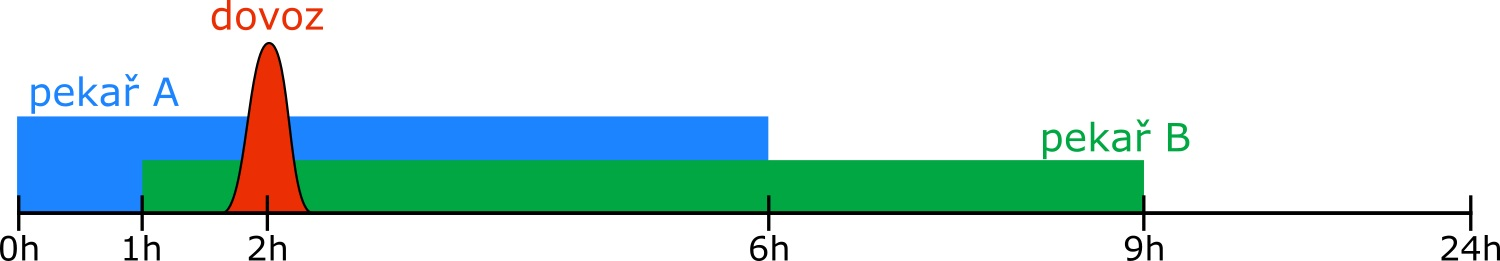
\includegraphics[width=\linewidth]{timeline.jpg}
  \caption{Průběh pracovní směny vyobrazen na časové ose}
  \label{fig:timeline}
\end{figure}

\subsection{Použité postupy}
Pro návrh Petriho sítě(~\cite{prezentace}, slajd X) byl použit vektorový grafický editor Inkscape a pro vytvoření modelu knihovna SIMLIB(~\cite{prezentace}, slajd 164) programovacího jazyku C++. Tato knihovna usnadňuje práci pro simulaci našeho zadání. 

\section{Koncepce modelu}
Cílem projektu je simulovat spolupráci dvou pekařů a zaznamenat jejich produktivitu. K simulaci není třeba brát ohled na množství prodaného pečiva, nebo dalšího zaměstnance obsluhujícího pokladnu. 

Zmínění pekaři mají přesně určené role, které vyplývají z běžné praxe, kdy jeden z pekařů se stará o přípravu těsta, zatímco druhý obsluhuje pece.

\subsection{Návrh konceptuálního modelu}
Simulace začíná v momentě nástupu prvního pekaře na směnu. Započne jeho osmi hodinová směna a pekař se dá do přípravy chlebu a následně rohlíků. Tento postup se opakuje až do konce jeho směny. Poté pekař opouští systém a vrací se znovu až za 16 hodin.

O hodinu později přichází druhý pekař. Rozdílný čas nástupu na směnu opět vychází z praktik v praxi. Druhý pekař by totiž čekal přibližně hodinu, až pekař první dokončí přípravu těsta. Jeho směna probíhá opakovaným pečením chlebu, rohlíků a kaiserek, které se dováží jednou denně zmražené. 

\subsection{Formy konceptuálního modelu}
Abstraktní(~\cite{prezentace}, slajd X) model(~\cite{prezentace}, slajd 7) byl popsán Petriho sítí(~\cite{prezentace}, slajd 123) podle informací získaných rozhovorem s naším odborníkem z oboru. 

\begin{figure}[H]
  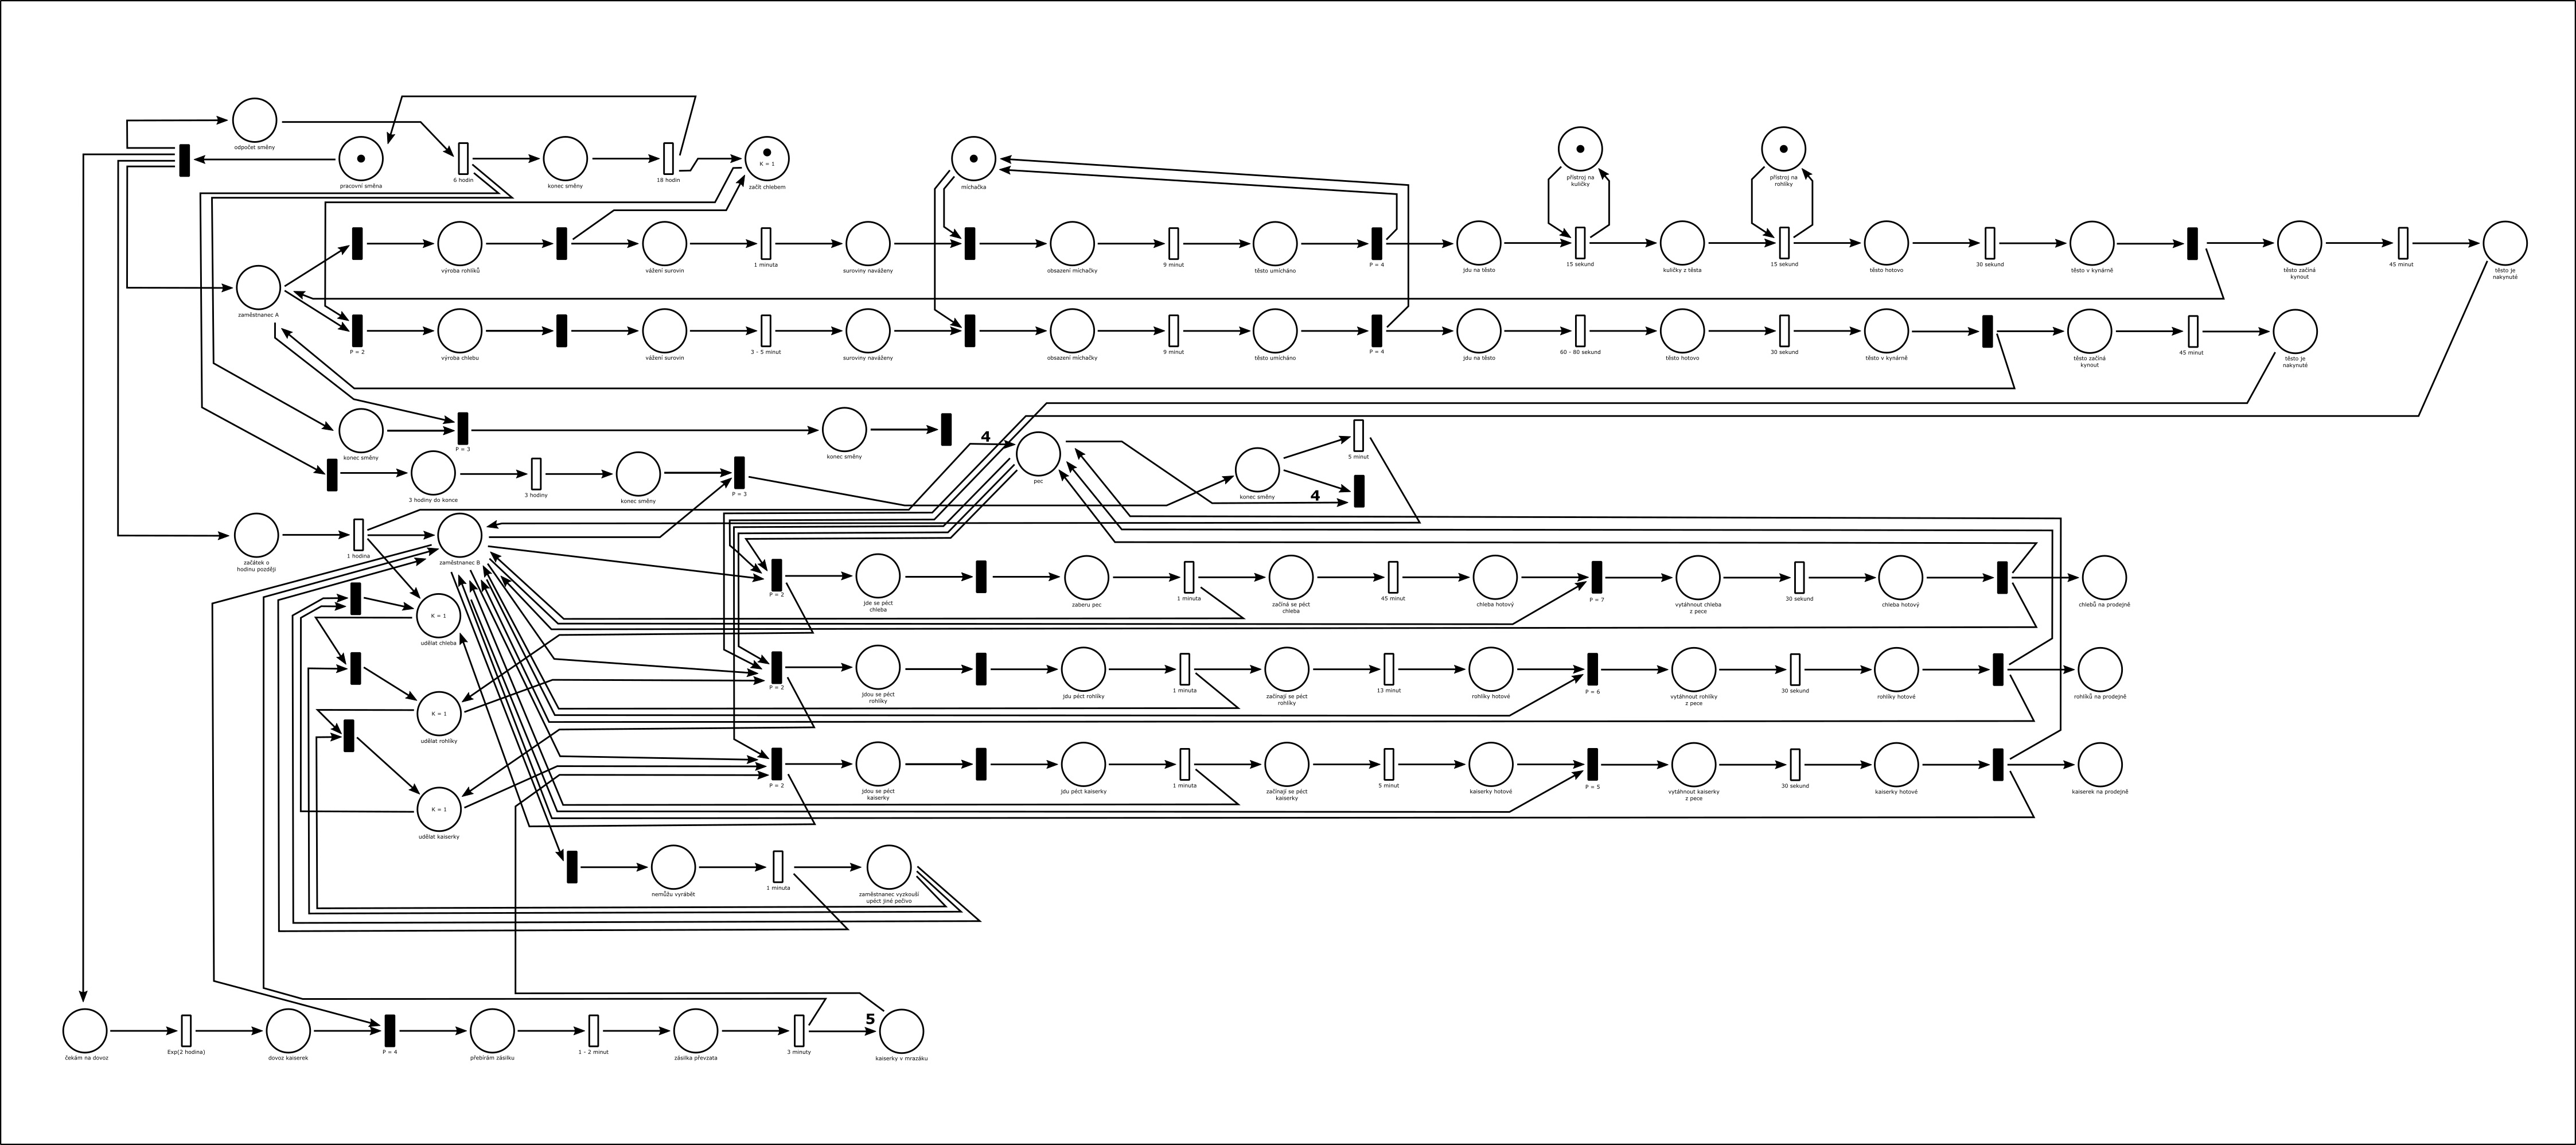
\includegraphics[width=\linewidth]{PetriNet.jpg}
  \caption{Petriho síť, viz příloha PetriNet.jpg}
  \label{fig:petrinet}
\end{figure}


\section{Architektura simulačního modelu}
Simulační model se sestává z tříd:
\begin{itemize}  
\item \verb|BapDoughImport| - proces dovozu mražených kaiserek
\item \verb|BakingBread| - proces pečení chlebu
\item \verb|BakingRolls| - proces pečení rohlíků
\item \verb|BakingBap| - proces pečení kaiserek
\item \verb|BreadDoughDries| - proces kynutí chlebu
\item \verb|RollsDoughDries| - proces kynutí rohlíků
\item \verb|WorkerAWork| - proces práce prvního pekaře
\item \verb|WorkerBWork| - proces práce druhého pekaře
\item \verb|WorkingShift| - proces pracovní směny
\end{itemize}

V hlavním bloku funkce \verb|main| je možnost pro vstupy označující množství odpracovaných směn a dostupných pecí. 


\section{Podstata simulačních experimentů a jejich průběh}
Původní testování probíhalo s údaji, kdy oba pracovníci měli stejně dlouhou směnu a k dispozici byly pouze dvě pece. Výsledky však ukázaly, že v takovémto případě není druhý pekař schopen upéct všechno těsto, které mu první pekař během pracovní směny připraví. Bylo tedy potřeba ovlivnit dva elementy v návrhu. A tím byla doba, po kterou pracuje první pekař. Z původních osmi hodin na šest. A zároveň zvednout množství dostupných pecí na 3. 

\subsection{Obecný popis simulačních experimentů}
Experimentování bylo provedeno měnícími se vstupními argumenty a porovnáváním výstupních hodnot.
\subsection{Jednotlivé experimenty}
\subsubsection{Experiment s množstvím pecí}
Prvním experimentem je pokus s měnícím se počtem pecí. Počet pecí výrazně ovlivňuje produktivitu druhého pekaře, zatímco prvního se to nijak nedotkne. S větším množstvím pecí je pekař schopen upéct více kusů pečiva. Výsledky jsou sčítány za 500 směn. 

\begin{figure}[H]
  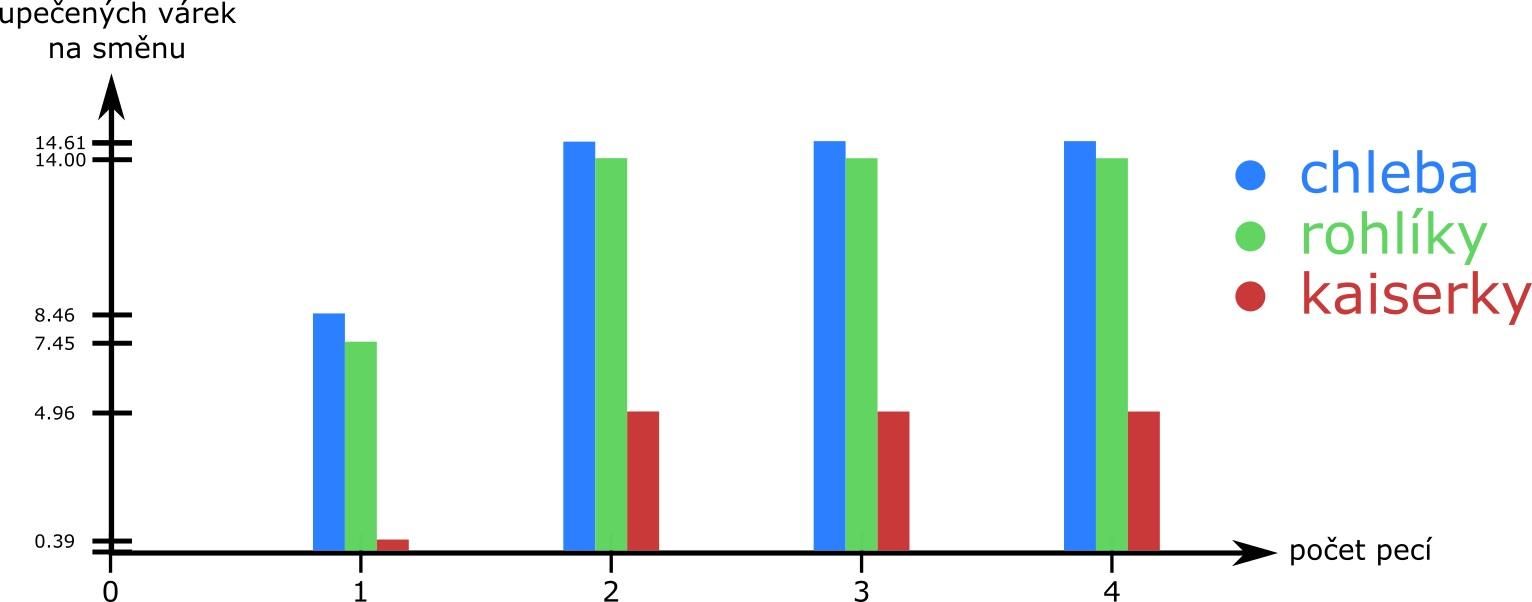
\includegraphics[width=\linewidth]{pece.jpg}
  \caption{Graf množství vyrobeného pečiva v závislosti na pecích}
  \label{fig:pece}
\end{figure}

\subsubsection{Experiment s počtem směn}
Druhý experiment zobrazuje množství upečeného pečiva za proměnlivý počet směn. Je vidět, že kvůli minimálnímu počtu proměnných ovlivňujících délku výroby (chleba se peče vždy stejně dlouho), nemáme veliké rozdíly v počtu vyrobených kusů na směnu. Můžeme si však všimnout, že v některých případech byli pekaři schopni vyrobit o jednu várku chleba více.

\begin{figure}[H]
  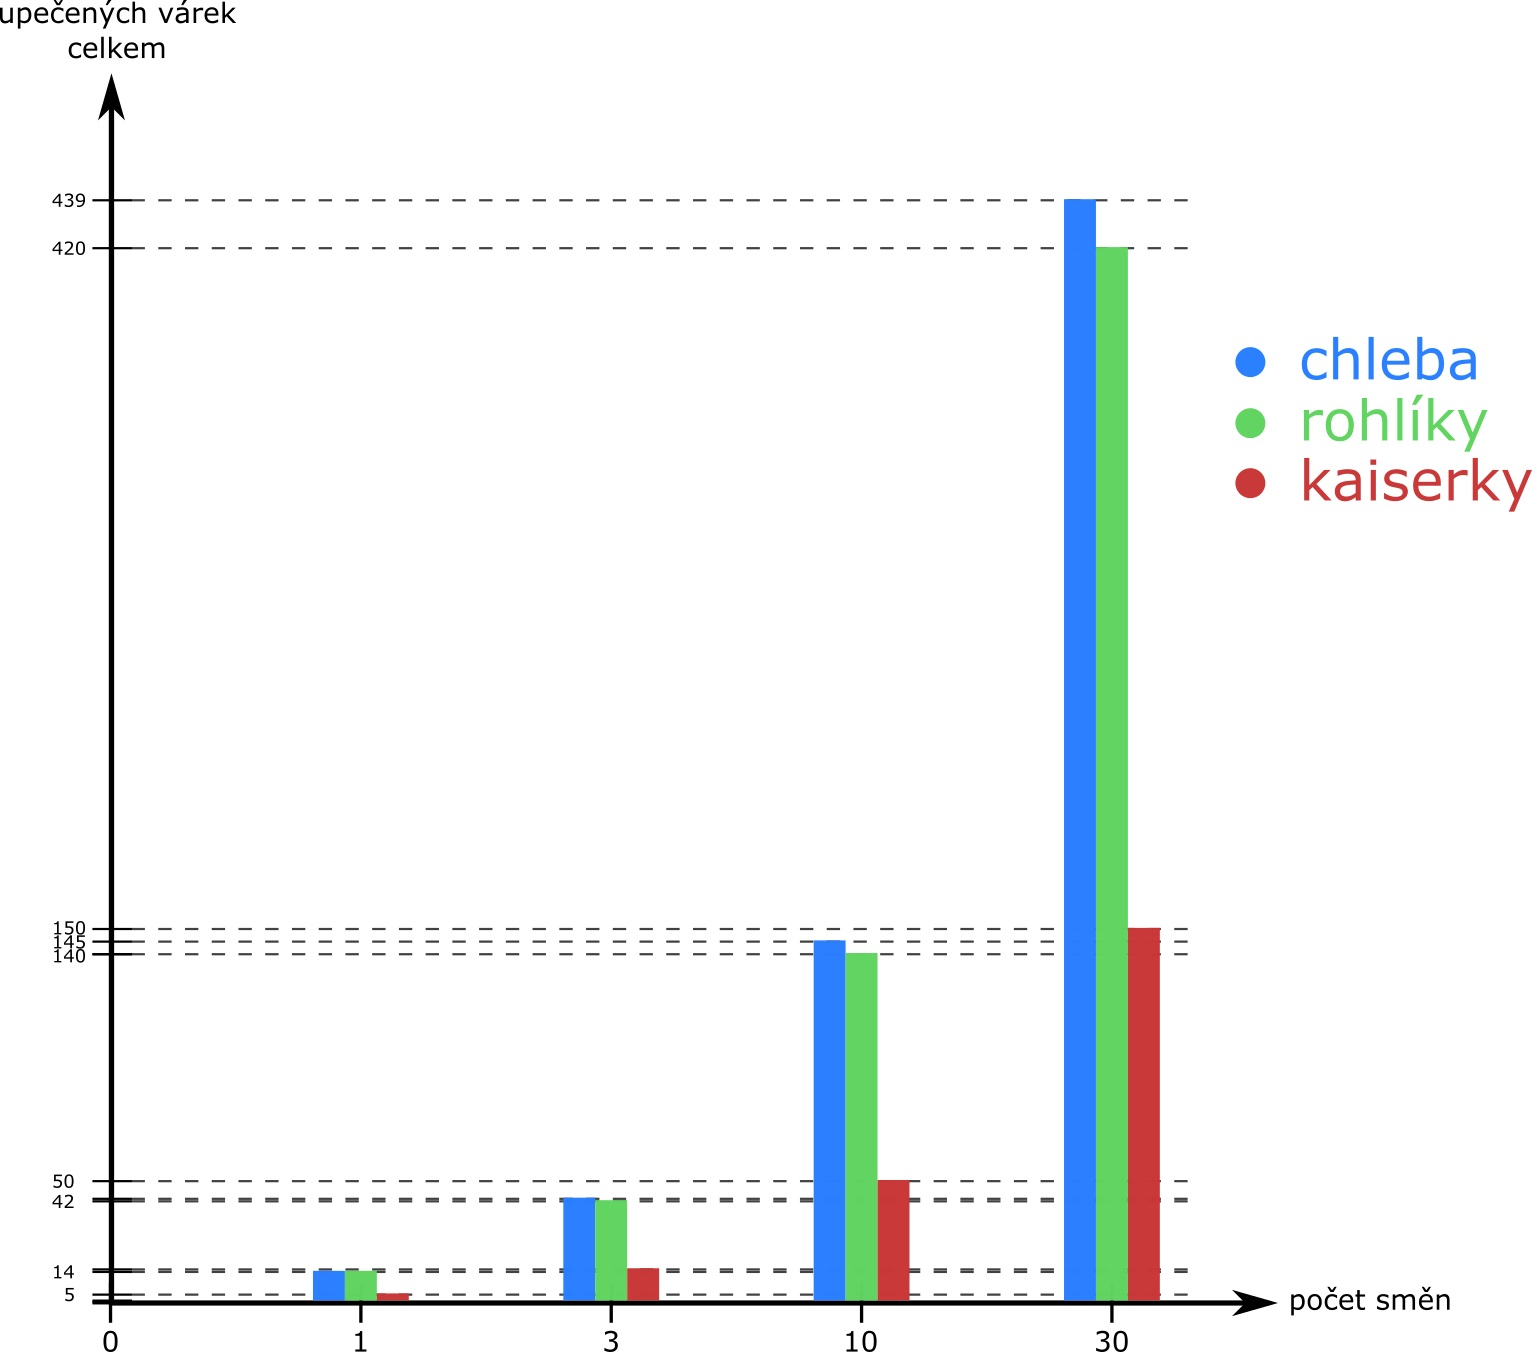
\includegraphics[width=\linewidth]{smeny.jpg}
  \caption{Graf množství vyrobeného pečiva v závislosti na směnách}
  \label{fig:smeny}
\end{figure}

\subsection{Závěr experimentů}
Byly provedeny 2 experimenty na jejichž základě byl upraven model změnou množství dostupných pecí a doby pracovní směny prvního pekaře. Z výše zobrazených výsledků lze vidět, že 3 pece druhému pekaři stačí pro bezproblémový chod pekárny.  

\section{Shrnutí simulačních experimentů a závěr}
Simulací zmíněných experimentů jsme zjistili množství pečiva, kterého jsou 2 pekaři při adekvátním počtu pecí dosáhnout. 

\newpage


\bibliography{manual}{}
\bibliographystyle{acm}
\end{document}

